\documentclass{article}
\usepackage[a4paper, margin=1in]{geometry}
\usepackage{datetime}
\usepackage{graphicx}
\newdate{date}{25}{1}{2022}
\date{January 25th 2022}

\usepackage{hyperref}
\usepackage{minted}

\title{Initiation to 3D Printing -- Practical exercises 3}
\author{Sylvain Lefebvre and Camille Schreck, ENSEM 2020-2021}

\begin{document}

\maketitle

\section{Important information}
\begin{itemize}
    \item The code can be written in either C, C++, Python, or JAVA language, your choice.
    \item At the end of the session, send the {\bfseries code and GCode of Exercise 3, 4 and 5 (optional bonus)} packed into a single ZIP file to:
          \begin{itemize}
        \item \href{mailto:sylvain.lefebvre@inria.fr}{sylvain.lefebvre@inria.fr}
        \item \href{mailto:camille.schreck@inria.fr}{camille.schreck@inria.fr}
    \end{itemize}
    with the mail subject {\bfseries ENSEM: TP3 [nom][prenom]}.
    \item {\bfseries Name your zip file: TP3\_[nom]\_[prenom].zip}.
    \item Before leaving the class, check with the professor that the mail with your ZIP was well received.
\end{itemize}

\section{Useful Links}

\begin{itemize}
	\item To write and test GCode \url{http://shapeforge.loria.fr/vrprinter}
	\item Another GCode viewer \url{http://gcode.ws}
	\item List of GCode instructions \url{http://marlinfw.org/meta/gcode/}
\end{itemize}

\section{Slicing algorithm}

Complete the slicing algorithm written during class (slicing.cc) but computing the correct value of E.

\section{Sparse filling a cube}

\subsection{Three sets of parallel lines in a square}

We are going to fill a square of $36 \times 36$ mm with three sets of parallel lines:

\begin{enumerate}
\item The first set is at a $45$ degree angle with a spacing of 4mm.

\begin{center}
\includegraphics[width=0.1\linewidth]{45deg.pdf}
\end{center}
\item The second set is at a $-45$ degrees angle with a spacing of 4mm.

\begin{center}
\includegraphics[width=0.1\linewidth]{315deg.pdf}
\end{center}
\item The last set is at an angle of $0$ degree angle with a spacing of 4mm.

\begin{center}
\includegraphics[width=0.1\linewidth]{0deg.pdf}
\end{center}
\end{enumerate}

Make sure the 4mm spacing can be adjusted from a variable.


\subsection{Progressive offset in the cube}

We are going to fill a cube of dimensions $36 \times 36 \times 36$ mm

Progressively offset the lines at each layer, moving them sideways (to their right) by half a nozzle (typically 0.2mm). Generate GCode. You should now see three sets of angled walls forming closed 3D cells. For an illustration and more information refer to this URL:

\url{http://sylefeb.blogspot.com/2015/07/3dprint-3d-infilling-faster-stronger.html}

\begin{center}
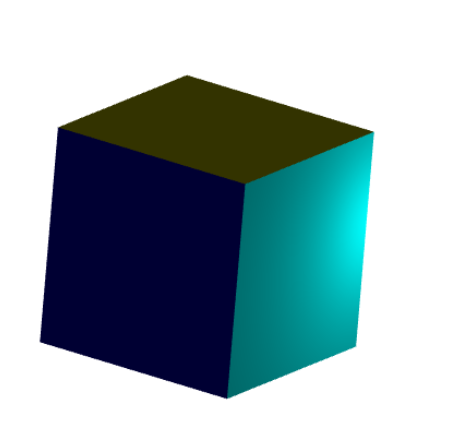
\includegraphics[width=0.25\linewidth]{cube.jpeg}
\end{center}

\section{Bonus: honeycomb infill}

Fill an square of $36 \times 36$ mm with a honeycomb infill:

\begin{center}
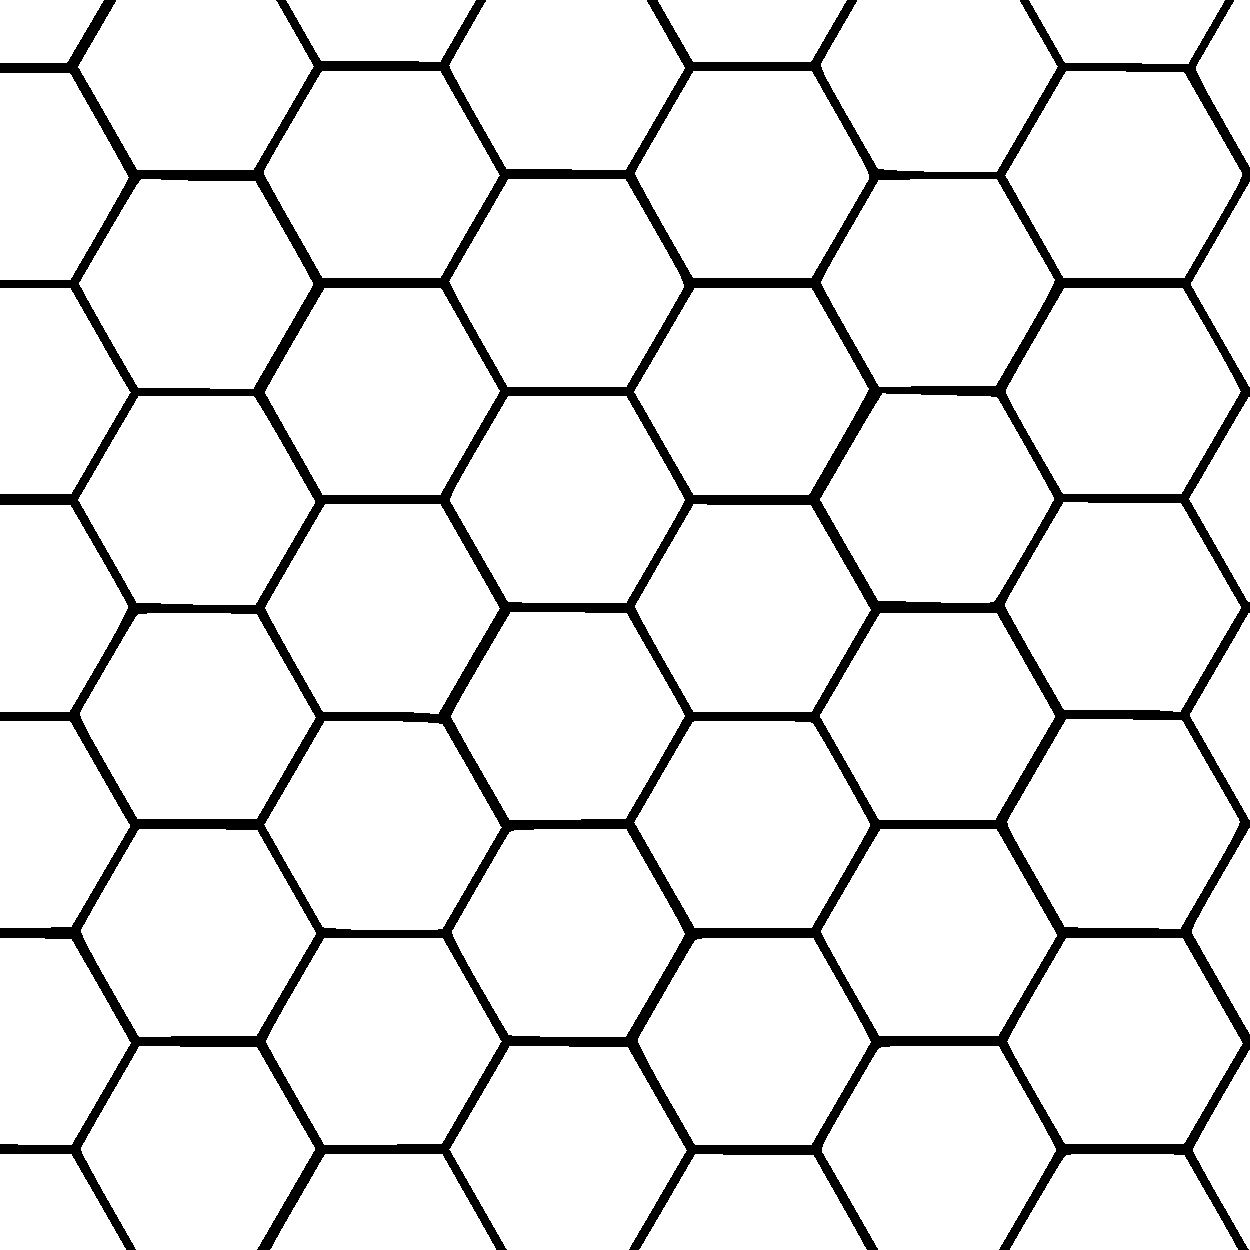
\includegraphics[width=0.25\linewidth]{honeycomb.pdf}
\end{center}

which is a periodic tiling of regular hexagonal polygons with circumradius $3$mm.

\section{Miscellaneous: sample code C++}

\begin{minted}{cpp}
#include <iostream>
#include <fstream>
#include <cmath>  // use constant M_PI to get the value of pi

int main () {
    std::ofstream file;
    file.open ("square.gcode");
    // header
    file << "G21" << std::endl;  // dimensions in milimeters
    file << "G90" << std::endl;  // absolute positioning
    file << "G28" << std::endl;  // homing

    // exercise code
    file.close();
    return 0;
}

\end{minted}

In Linux, compile the above program (contained in a file main.cpp) with:

\begin{minted}{bash}
g++ main.cpp -o main
\end{minted}

\end{document}

